\chapter{Case Studies}

%short introduction
%one section for each one of the case studies
%general structure for each one of the sections
    %1) Description of the model with Event-B code
    %2) Results of the simulation

The purpose of these case studies is to test the correct integration of the encoder with the MultiVeStA tool. In total there are 3 case studies: two probabilistic programs using dices and coins, a bounded re-transmission protocol, and a program that simulates a modal operator in positive negative logic. The repository that contains the code of this integration can be found in the following repository: \url{https://github.com/dfosorio/EventB2Maude-MultiVeStA}. Furthermore, this repository contains the code of the probabilistic Event-B models, their translated versions in PMaude, and the results of the simulations. An short guide on how to use the software can also be found in this repository, for any reader that might want to test or use the tool.



\section{Dice Programs}
The dice programs, based on the Knuth \& Yao paper \cite{knuth}, were originally discovered in the PRISM model checker web page \cite{PRISMDICE}. The idea is then to translate the model from the PRISM language to probabilistic Event-B. Then, the probabilistic Event-B model can be translated into PMaude using the encoder, and verified using MultiVeStA. If the results from the MultiVeStA simulations are the same as the PRISM model checker, then we can assume that the encoding and verification process were performed correctly. The probabilistic model for the first dice program is the following:
\begin{figure}[H]
    \centering
    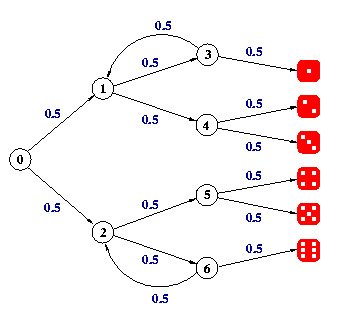
\includegraphics[scale = 0.5]{images/CE1.png}
    \caption{States and transitions of the dice model, taken from \cite{PRISMDICE}}
    \label{fig:ce1}
\end{figure}
Having as a reference the Figure \ref{fig:ce1}, the starting state of the model is the state 0. Afterwards a fair coin is tossed to decide the next transition to execute. If the coin lands on heads, then the upper branch is taken. Conversely, when the coin lands on tails, the lower branch is taken. This process is repeated in each on of the sates 1 to 6, until reaching a terminating state, i.e. reaching a state where one of the dice faces is chosen. To represent this model in probabilistic Event-B, the process is straight forward: to represent all the states of the model a deferred set with all is created in the context.
\begin{maude}

CONTEXT ctxDiceProgram1
SETS 
    STATES : { s0, s1, s2, s3, s4, s5, s6, s7 }
CONSTANTS 
END
\end{maude}
where the state $s_7$ represents all the possible terminating states. In the machine of the model, two variables will be considered: one that stores the current state of the system and other that contains the current value of the dice.
\begin{maude}

MACHINE DiceProgram1
  SEES ctxDiceProgram1
  
  VARIABLES
    st 
    dice 
  INVARIANTS
    st : STATES
    dice : Nat 
\end{maude}
Each one of the transitions or coin tosses is represented with an event. For example, the first two transitions that start in state 0 can be represented with the event:
\begin{maude}

EVENT State0Trans 
WEIGHT 1
WHERE 
    st = s0
THEN
    st := {s1 @ 0.5 , s2 @ 0.5 }
END
\end{maude}
As seen in the event, fifty-fifty probability of the coin toss is represented with a probabilistic assignment. For transitions that precede a terminating state, they are represented by changing the state to $s_7$, and assigning to the dice the respective value. For example, the transitions that branch out of the fourth state are represented in Event-B as:
\begin{maude}

EVENT State4Trans 
WEIGHT 1
WHERE 
    st = s4
THEN
    st := s7
    dice := {2 @ 0.5 , 3 @ 0.5 }
END    
\end{maude}
Finally, to initilize the system the values $s_0$ and 0 are assigned to the variables $st$ and $dice$ respectively.
\begin{maude}

INITIALISATION
    st := s0
    dice := 0
\end{maude}


The property that wants to be verified for this program is the probability of reaching a value of $dice = k$, where $k = 1,2,...,6$. 

    